\section{Matched local-designer comparison with stronger references}
\label{sec:matched}
The preceding cases establish executable freedoms and bounded observations,
but differ in source, author and feedback. They cannot answer whether a local
code/graph designer outperforms parameter tuning. V2 therefore fixes one native
source and compares proposal packages prospectively. It is complementary
evidence, not a replacement for the earlier structural and gradient questions.

\subsection{Objectives, domains and information boundaries}
The study uses five researchers, fixed Qwen3-8B scientist weights, a four-year
CS literature corpus, two-year development worlds and common world seed 42.
The primary minimized losses are
\begin{equation}
 T=-A,\qquad C=4A-Q+0.1R.
\end{equation}
The earlier $E=-Q+0.5R$ is diagnostic only, not a third search arm. The older
$U=3.25A-Q+0.05R$ remains a different study's objective. No coefficient is
retuned from V2 results. The common editable seed is not the untouched legacy
institution; both are evaluated separately.

Each primary objective has five proposal policies:
\begin{enumerate}[leftmargin=*,nosep]
 \item LLM numeric: six declared coordinates, fixed source and topology.
 \item LLM code/fixed graph: those coordinates and three existing Python bodies.
 \item LLM code/graph: any valid specification within the native study contract.
 \item Technical-only code/graph: the same broad domain without scientific-loss
 feedback, using the fixed initial parent and its own technical history.
 \item Uniform numeric: independent samples of the same six coordinates, without
 a designer-model call.
\end{enumerate}
The six coordinates are two existing tensor thresholds, bias, memory cost,
router threshold and integer process count. Domains are checked against the
initial anchor, not the previous parent, so gradual edits cannot escape a
restricted arm. The code/graph domain permits structure change but cannot
change scientist weights, corpus or measurement functions.

All LLM arms use the same approved local 35B designer profile: 16 charged actions,
8192 output tokens, 40960 context, temperature 0.6, thinking off, 10s connect/900s
read allowances, without hidden transport retry or slot refill. Technical
errors expose the same exception-class channel. Three fresh controller
histories, each four generations per arm, give 120 candidate slots. Controller
seeds 42/1031/2063 are not independent development worlds: every forward still
uses world seed 42. Reference results and other arms' histories are not supplied
to the designer. Fresh source/model/backend-bound interface controls precede
dispatch; exact-copy equality is diagnostic, not a merit criterion.

Technical-only filtering hides losses, measurements, loss-selected parents,
incumbent indicators and derived outcome metadata, not merely the scalar text.
The intervention therefore includes parent selection, not only score display.
Technical success remains visible and may itself be informative. This is a
bounded information policy, not an adversarial isolation theorem about the
entire operating environment.

\subsection{References, selection and unused conditions}
Nine fresh references share the same source/world: legacy, editable seed,
rank/rate, all-accept, all-reject, score thresholds 3/4 and reviewer-free
accept/reject. Earlier S1 controls are not reused as these fresh observations.
These references prevent attributing a weak-seed improvement to successful
invention when an obvious rule already achieves it.

After all search slots, each objective/arm chooses from every completed
candidate plus the initial system using only its declared loss. Every exact
tie is retained; the earliest declared chronology supplies the representative.
An initial selection is reported as no discovered improvement, not a generated
replacement for failed proposals. The selection manifest is frozen before
unused-condition evaluation and its results never return to search.

The 19 logical labels comprise 15 exact policies. Explicit sharing gives 90
physical jobs: each policy on five unused seeds 31001/31013/31019/31033/31039
for two years, plus a separate four-year diagnostic at 31001. Shared labels
do not create independent samples; four years is not pooled with the five
two-year observations. All 90 jobs finish normally.

\subsection{All attempts, paths and exercised freedoms}
% Generated from CLOSED report 75f64370d673699553f69c480c93b90c07c2babba70b4f924cbc54438ab9d732
\begin{table}[t]
\centering\small
\begin{tabular}{@{}llrrrrrr@{}}
\toprule
Obj. & Proposal space/control & Meas. & G-null & X-null & M-null & Best & Ties\\
\midrule
$T$ & LLM numeric & 0/12 & 12 & 0 & 0 & 0.000$^{\ast}$ & 1\\
$T$ & LLM code, fixed graph & 9/12 & 1 & 2 & 0 & -7.000 & 9\\
$T$ & LLM code and graph & 7/12 & 0 & 5 & 0 & -7.000 & 6\\
$T$ & Technical-only code/graph & 7/12 & 0 & 5 & 0 & -7.000 & 5\\
$T$ & Uniform numeric & 12/12 & 0 & 0 & 0 & -7.000 & 8\\
\midrule
$C$ & LLM numeric & 0/12 & 12 & 0 & 0 & 2.400$^{\ast}$ & 1\\
$C$ & LLM code, fixed graph & 6/12 & 0 & 6 & 0 & 2.100 & 2\\
$C$ & LLM code and graph & 8/12 & 0 & 4 & 0 & 2.100 & 2\\
$C$ & Technical-only code/graph & 3/12 & 0 & 9 & 0 & 2.400$^{\ast}$ & 3\\
$C$ & Uniform numeric & 12/12 & 0 & 0 & 0 & 2.400$^{\ast}$ & 4\\
\bottomrule
\end{tabular}
\caption{\textbf{All scheduled development attempts.} Each row pools three
controller histories with four proposals each, all at world seed~42.
Meas.: available assigned losses; G/X-null: generation/execution failures;
M-null: completed forward with unavailable assigned loss. Nulls are not penalties.
Best includes the shared initial system; $\ast$ marks its selection, not an invention.
Ties count all exact minimizers, including the initial reference when tied.
Only display values are rounded; selection uses unrounded report values.
Controller histories are not independent environment replications.
}
\label{tab:v2-search-outcomes}
\end{table}

Of 120 slots, 64 complete, 25 fail generation and 31 fail execution.
All 24 uniform numeric proposals execute; all 24 LLM numeric proposals exhaust
their action budget without a valid explicit submission. One fixed-graph code
proposal also fails generation. The technical nulls are not numeric bad losses.

A bounded inspection confirms the correct six-coordinate contract in all 24
initial numeric-arm HTTP requests, with initial prompt counts 12145--12411,
40960 context and 8192 output settings without truncation. The general editor
protocol and restricted session domain coexist. This refutes the narrow claim
that the contract was absent; it does not establish clear salience, comprehension,
later-call capacity or the cause of every failure. The end-to-end comparison
therefore includes interface compliance and does not isolate intrinsic
expressivity. Literal error categories appear in Appendix~\ref{app:failures}.

Full-spec inspection joins all 64 complete candidates and all frozen ties.
Forty candidates change selection source, and others change existing numeric
settings. None changes declared node IDs/order, wiring, node ABI, initial state
or schedules. Twenty change numeric process count, so unchanged graph metadata
is not proof of unchanged runtime behavior. The code/graph label denotes
permission, not a structural invention observed in this study.

\begin{figure}[p]\centering
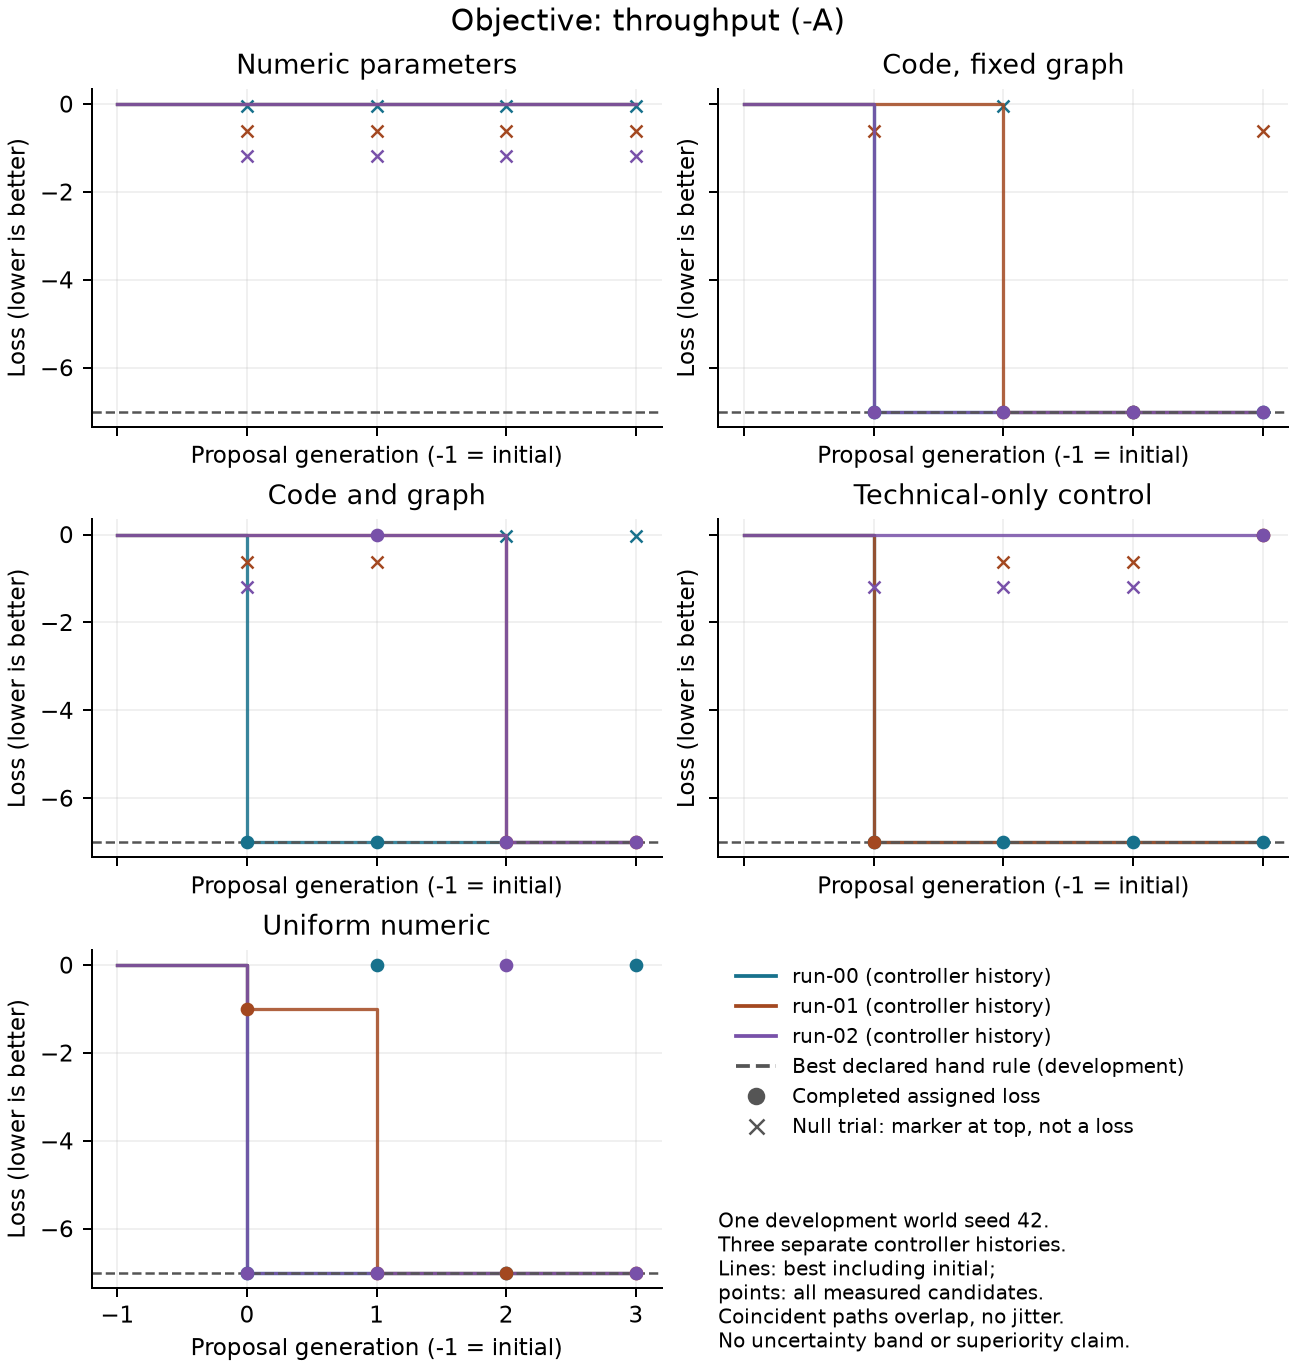
\includegraphics[width=\linewidth,height=.80\textheight,keepaspectratio]{figures/native-design-v2/throughput-paths.png}
\caption{\textbf{All V2 throughput histories.} Every measured candidate and
generation/runtime null remains. Lines show best including the shared initial
observation; a line through a null does not make that attempt successful.
The hand-rule line is a stronger reference, not an extra objective or veto.
Three controller histories use the same development world seed.}
\label{fig:integrated-v2-t}
\end{figure}
\begin{figure}[p]\centering
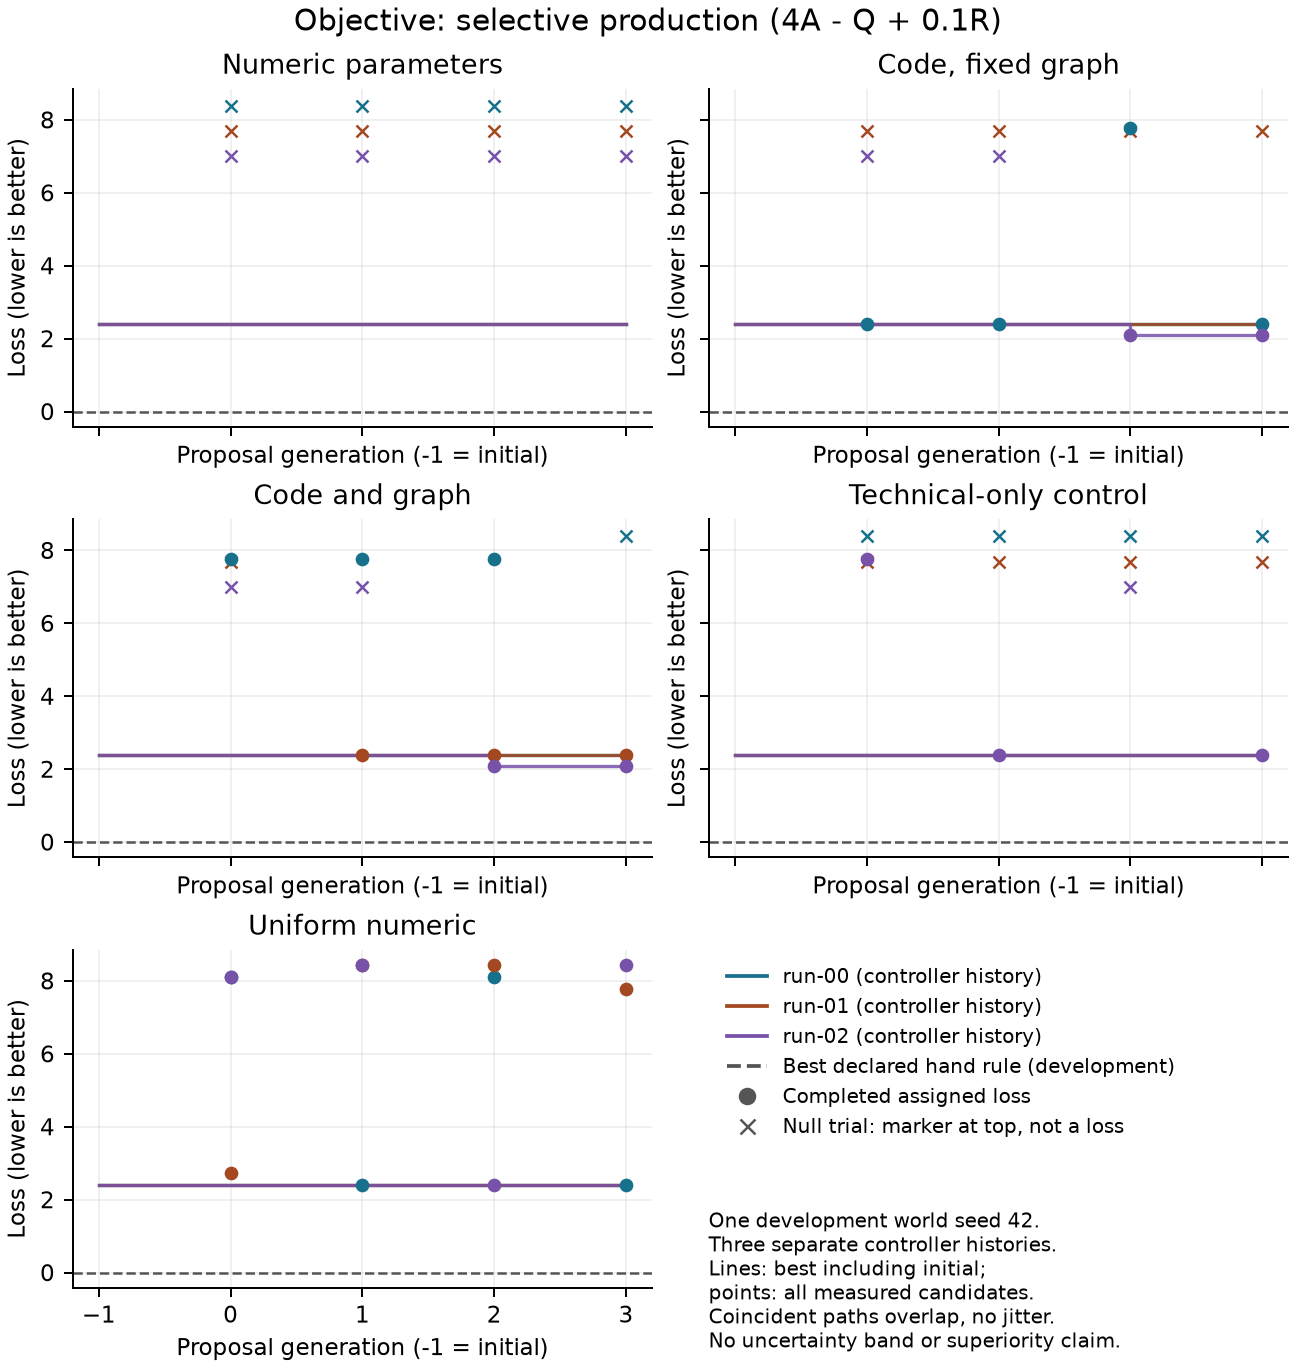
\includegraphics[width=\linewidth,height=.80\textheight,keepaspectratio]{figures/native-design-v2/selective-paths.png}
\caption{\textbf{All V2 review-cost-sensitive histories.} Code minima improve
editable initial 2.4 to 2.1, but not reviewer-free reject 0. Uniform and technical-only
controls are retained even when they tie or do not improve. Own-loss units are
not comparable to the throughput panel's units.}
\label{fig:integrated-v2-c}
\end{figure}

Throughput repeatedly reaches $T=-7$, matching all-accept at development seed 42.
Uniform numeric and technical-only proposals also reach it. For $C$, code
minima 2.1 improve editable initial 2.4 but not reviewer-free reject 0.
Initial policies are selected for both LLM numeric arms and for $C$ technical-only
and uniform arms. The whole path, rather than its most favorable history,
provides no evidence of feedback or free-design superiority.

\subsection{Selected policies under common evaluation scores}
Figure~\ref{fig:integrated-v2-cross} reports every reference and selected label
under common $T/C/E$. Executable throughput code/control and uniform selections
average 6.2 acceptances over five unused two-year seeds, matching all-accept
and score 3. Legacy averages 2.6 and the editable seed 0.2. Reviewer-free
accept-all also averages 6.2, with $Q=R=0$: equal throughput is not equal
review-backed production or better science.

Both $C$ code selections have mean $A=Q=0,R=19.2$, hence mean $C=1.92$.
Editable seed and review-based reject-all each average 2.58; reviewer-free
reject remains 0. Diagnostic mean $E=9.6$ is not favorable reviewed production.
The different objective selects different observed acceptance/review behavior,
but these data do not identify a novel optimal policy.

\begin{figure}[p]\centering
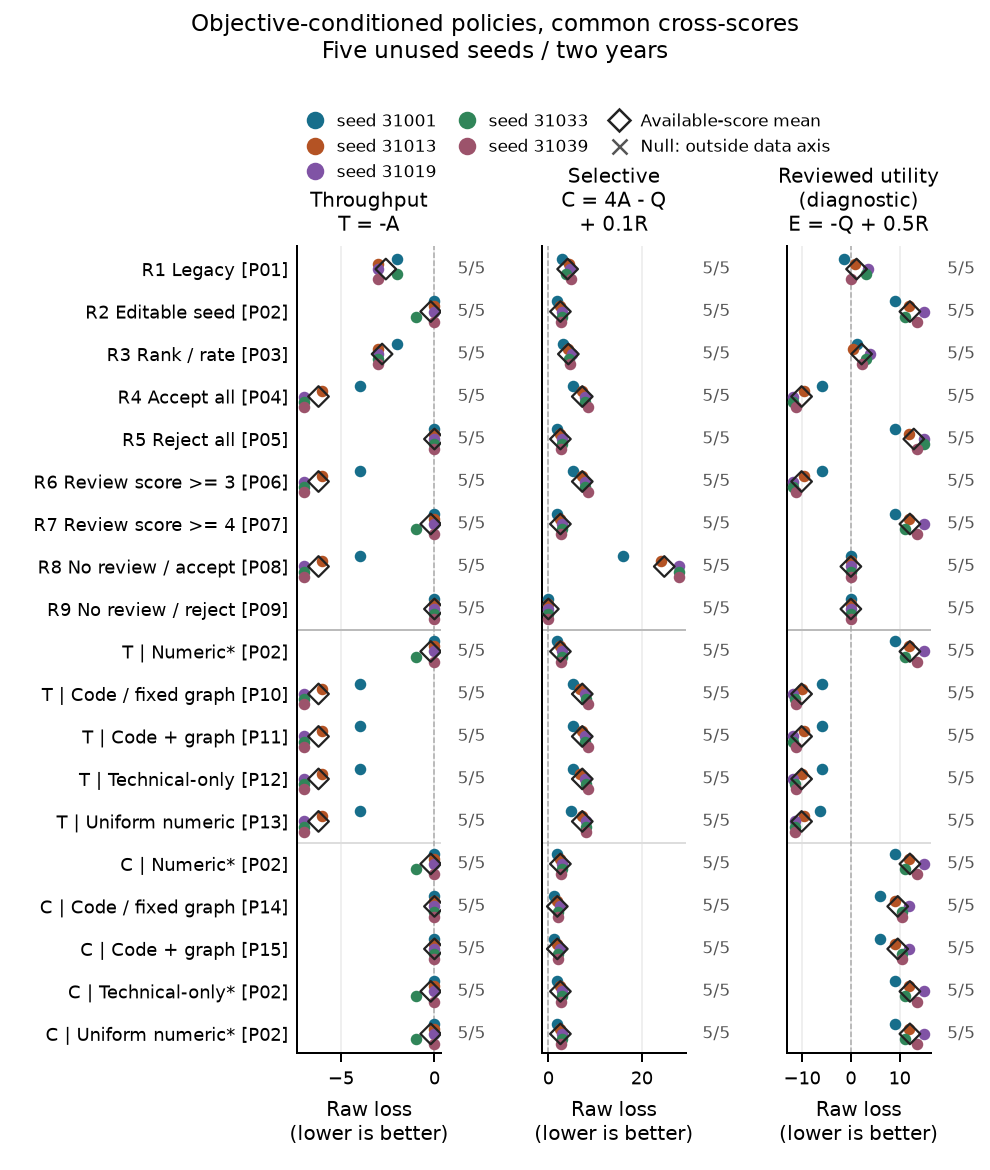
\includegraphics[width=\linewidth,height=.80\textheight,keepaspectratio]{figures/native-design-v2/cross-objective-2y.png}
\caption{\textbf{All selection-fixed V2 policies on five unused two-year seeds.}
Points are raw world observations; hollow diamonds are descriptive means, not
confidence intervals. Separate loss scales are neither normalized nor averaged.
P labels mark exact policy/job sharing, and stars mark initial selections.
E is diagnostic, not an E-optimized experiment.}
\label{fig:integrated-v2-cross}
\end{figure}

At the separate four-year seed, throughput executable selections and all-accept
each produce 11 acceptances. Both $C$ code selections have $A=Q=0,R=33$,
giving $C=3.3$, versus initial 6.9 and reviewer-free reject 0. Some equal-throughput
policies differ under $E$. One fresh four-year realization is not another
five-seed estimate or an isolated method effect.

\subsection{Mechanisms behind equal scalar losses}
The development $C=2.1$ selections have different components: code/graph gives
$A=Q=0,R=21$, whereas fixed-graph gives $A=1,Q=4,R=21$ and $4A-Q$ cancels.
An authored final score 0 is not the original-review measurement $Q$.
One fixed-graph history's G2/G3 sources have different bytes but equal Python
ASTs and otherwise equal specifications. Both keep their actual costs and
evaluations: AST deduplication was not a selection rule.

The selected $C$ code/graph program rejects addressed papers and writes final
score 0. The kernel applies that result to the actual paper, publication stores
it in review history, and the researcher resubmission prompt prints it. Three
audited year 2 requests contain the corresponding year 1 paper and score 0.00;
each joins one completed response with an empty resubmission list.
This traces an exercised program--record--input--action path. It does not
isolate score 0 as the cause of fewer reviews: no alternate intervention world
is simulated, and fresh LLM realizations are not perfectly coupled.

The distinction matters for future experiments. A generated parameter without
a consumer is inert; a changed consumer can affect future behavior even if
the graph is unchanged; equal losses need not imply equal institutions.
Source, actual input/output receipts and downstream state are needed together.
Unexercised empty-input or dummy-ID branches do not become validated because
one trajectory completes.

\subsection{Costs and outside metrics}
The writer's normal execution lasts 78958.697204 s, approximately 21 h 56 min.
Across the 194 physical response journals, 16043 recorded scientist responses
contain 17021423 total tokens. Proposal authoring records 1387 requests and
1385 final-response signals, not 1385 successful candidate submissions.
Its 19681.867535932688 host model-call seconds are a component, not GPU time
or an additive end-to-end compute total.293 role loads have unknown native
usage rather than zero usage. Appendix~\ref{app:costs} separates all scopes.

Search uses 95 world directories: 64 complete and 31 partial runtime-null worlds;
25 generation-null slots dispatch no native world. All 64 completed development
worlds and 90 evaluation jobs end with five active original researchers.
That final snapshot gives no observed separation, not equal lifetime careers.
Resources vary descriptively: two-year summed means are 616 for initial, 627
for $C$ code and 632 for throughput uniform, with overlapping ranges.
These endogenous resources are not money, welfare or a new optimization target.

\FloatBarrier
\section{A game-like observatory over the same research world}
\label{sec:observatory}
The interface is part of the research program, not a separate fictional
simulator. An English pixel/cyberpunk city provides a spatial view of
researchers and institutions; the Institution Foundry exposes source,
mechanisms, wiring, conditional distributions, losses and all attempts.
Canonical event/replay exports and verified checkpoints supply the numerical
state. The visual language makes the ecosystem inspectable without making
artistic choreography a measured research trajectory.

\begin{figure}[t]\centering
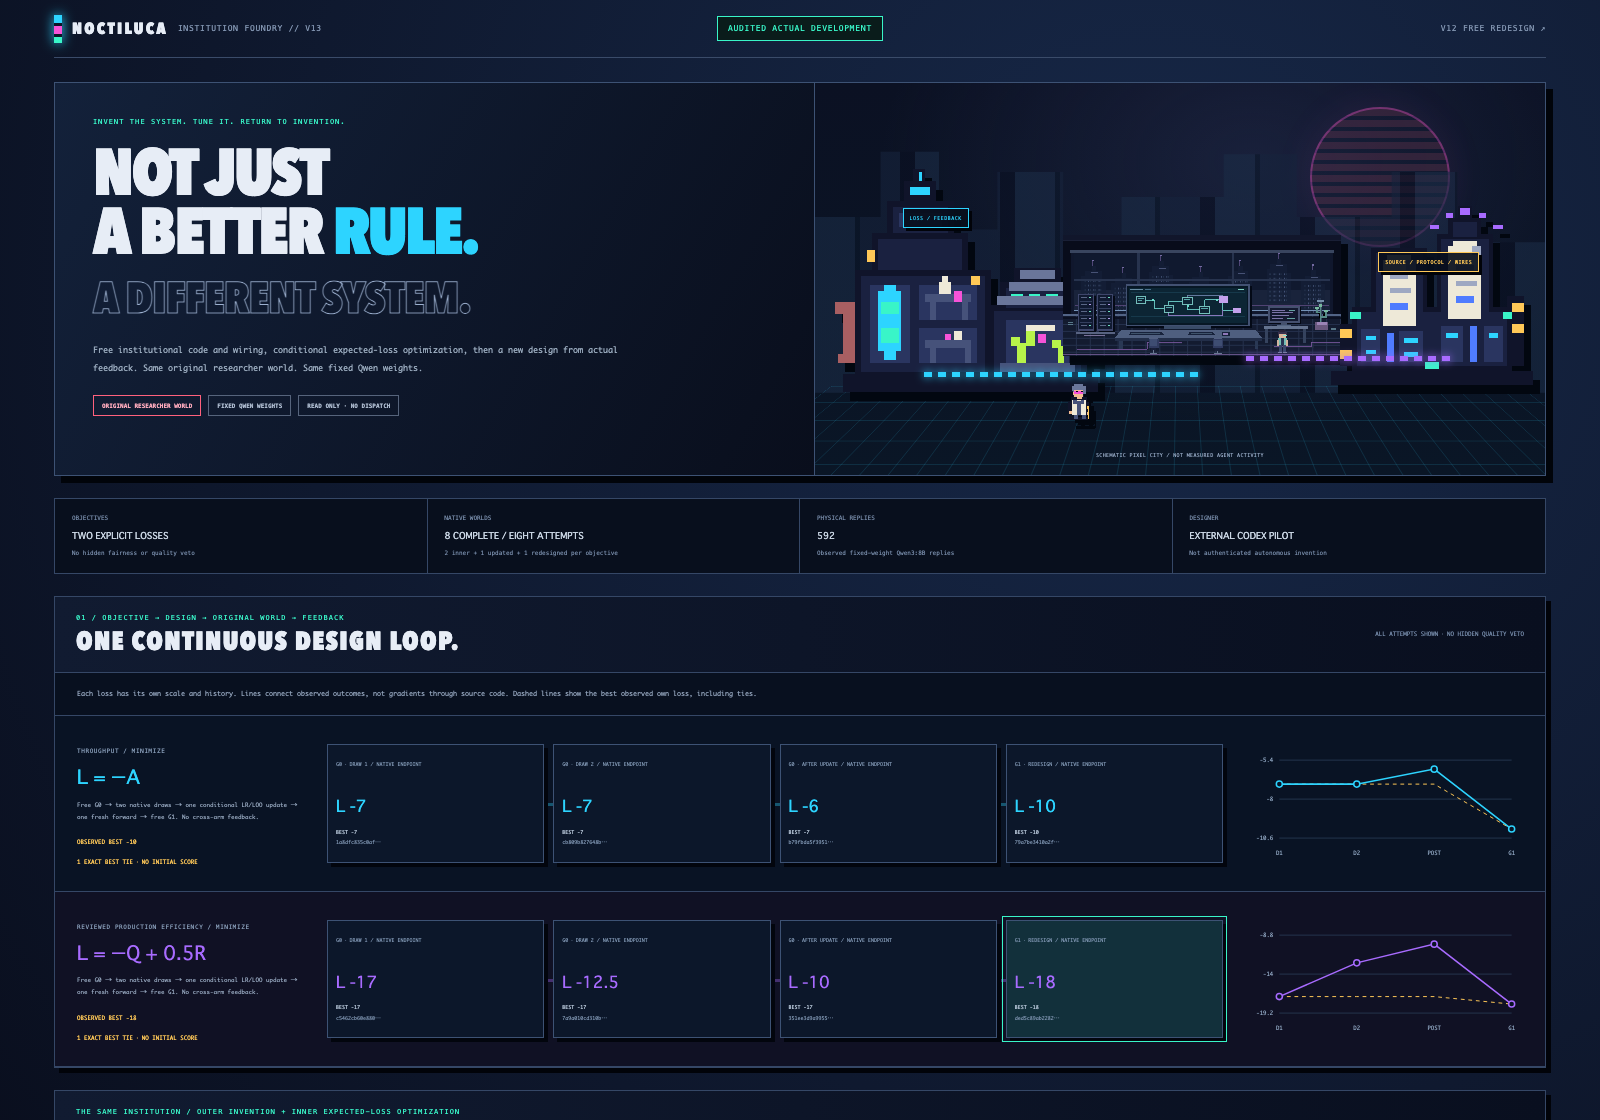
\includegraphics[width=\linewidth]{../game-ui-v2/screenshots/nested-foundry-v13-actual-qa/nested-foundry-v13-actual-overview.png}
\caption{\textbf{Actual English Institution Foundry view of the V13 evidence.}
Cards show the complete eight-world nested case, including worse post-update
draws and external-designer provenance. Pixel city movement is schematic, not
measured researcher motion. This historical capture is bound to V13, not a
claim that the screen displays the later V2 study or that gameplay improves
research understanding. Full-size captures remain in the artifact repository.}
\label{fig:integrated-ui}
\end{figure}

The useful interaction is to move between levels: inspect an objective's
history, select an observation, read the literal institution, follow its graph
and examine which effects reached native scientists. A local editable branch
can start from an observed system; a draft is not executed merely because it
is visible. Runtime validation, an explicit queued job and actual compute
authorization remain separate. Likewise, installing a new institution into
a continuing society is different from evaluating it in a reset world.

This establishes an evidence-reading and design interface, not a completed
management game. No user study, learning benefit, enjoyable gameplay or human
policy-design advantage is demonstrated. Those require separate evaluation.
The longer-term game can make information circulation and institutional
decisions interactive, but it must retain the same identity/state boundary
rather than manufacture a more flattering world for display.
\FloatBarrier
